\documentclass[oneside]{book}
\usepackage[english]{babel}
\usepackage[letterpaper,top=2cm,bottom=2cm,left=3cm,right=3cm,marginparwidth=1.75cm]{geometry}
\usepackage{amsmath}
\usepackage{graphicx}
\usepackage[colorlinks=true, allcolors=blue]{hyperref}
\usepackage{multirow}
\usepackage{multicol}
\usepackage{soul}
\usepackage{minted}
\usemintedstyle{perldoc}
\usepackage{listings}
\usepackage{markdown}

\setminted[cpp] {
    style=friendly,
    fontfamily=tt,
    linenos,
    autogobble,
    breaklines,
    numbersep=2pt,
    %framesep=2mm,
    bgcolor=white,
    fontsize=\small,
    escapeinside=||,
}
\lstdefinestyle{cpp}{
  belowcaptionskip=1\baselineskip,
  breaklines=true,
  xleftmargin=\parindent,
  language=C,
  showstringspaces=false,
  basicstyle=\footnotesize\ttfamily,
  keywordstyle=\bfseries\color{green!40!black},
  commentstyle=\itshape\color{purple!40!black},
  identifierstyle=\color{blue},
  stringstyle=\color{orange},
  numbers=left,
  stepnumber=1,
}
\lstset{escapechar=@,style=cpp}

\newenvironment{psmallmatrix}
  {\left(\begin{smallmatrix}}
  {\end{smallmatrix}\right)}
  
\setcounter{tocdepth}{4}
\setcounter{secnumdepth}{4}

\title{T2SP Programming Guide}
\author{Hongbo Rong}

\begin{document}
\maketitle

\tableofcontents
\lstlistoflistings

\chapter{Overview}

T2SP generates accelerators for dense tensor computes, and a general workflow is shown in Fig.~\ref{fig:overall-flow}. Usually, such a compute is described as one or a few math equations.  We can rewrite these equations to be recursive, the so-called Uniform Recursive Equations or UREs. With UREs, we can accurately control input and output data to flow in a pipeline fashion during the compute.

We can write basic UREs without tiling the compute domain. Then we tile the compute domain for data locality and reuse. Correspondingly, we need translate the basic UREs into final UREs after tiling, which is straightforward.

UREs can be expressed in C/C++. After adding some helper code necessary for testing,  we can compile them in a standard C/C++ compiler, and check if the UREs are correct vs. the original math equations.

The compute domain is iterated with a loop nest. If the compute is to run on a GPU, we need decide which loops are block loops, and inside a block, which loops are thread loops: An iteration of the thread loops will be turned into a thread. If the compute is to run on an FPGA, however, we always use a single thread for the entire compute, and thus there is no block or thread loop. 

Inside a thread, we will build a systolic array in a space-time transform. So we need decide which loops are space loops.  

Finally, we add an I/O network for the systolic array.  The I/O network is composed of multiple memory levels. The input/output data are loaded/unloaded through the I/O network into/out of the systolic array. Once in the systolic array, the data flow through the array according to the UREs.  

Now for the original compute, we have a complete T2SP program, or more accurately, a specification, since such a program only specifies what to implement (e.g. space-time transform and I/O network), but leave the actual implementation to the T2SP compiler. In other words, the program controls the compiler to generate the expected accelerator. 

For an FPGA, the T2SP compiler generates OpenCL device code and a C interface, compile and run these generated code by invoking the downstream FPGA tools. The programmer can use the emulator tool to verify correctness of the generated code, and use the synthesis tool to produce a bit-stream.  The programmer can write CPU host code and call the device code through the C interface, just like calling any normal C function on a CPU. That call would offload the compute to the emulator or an actual FPGA to run.

For a GPU, the T2SP compiler generates CM device code, and invoke the CM compiler to build a binary. The programmer need write CPU host code that offloads the device code to a GPU. 

A beginner might encounter several hurdles in using T2SP: (1) how to write UREs? (2) how to tile loops? (3) how to decide block, thread, and space loops? and (4) how to design I/O? There are numerous valid answers for each of these questions. Fortunately, we do not have to be mathematicians, algorithm experts, or computer architects in order to effectively address the questions. Based on intuitive rules, any programmer may master some simple programming skills quickly, and  use the skills to accelerate real-world workloads.

We will describe the steps in more details below. 

\begin{figure}[!ht]
    \centering
    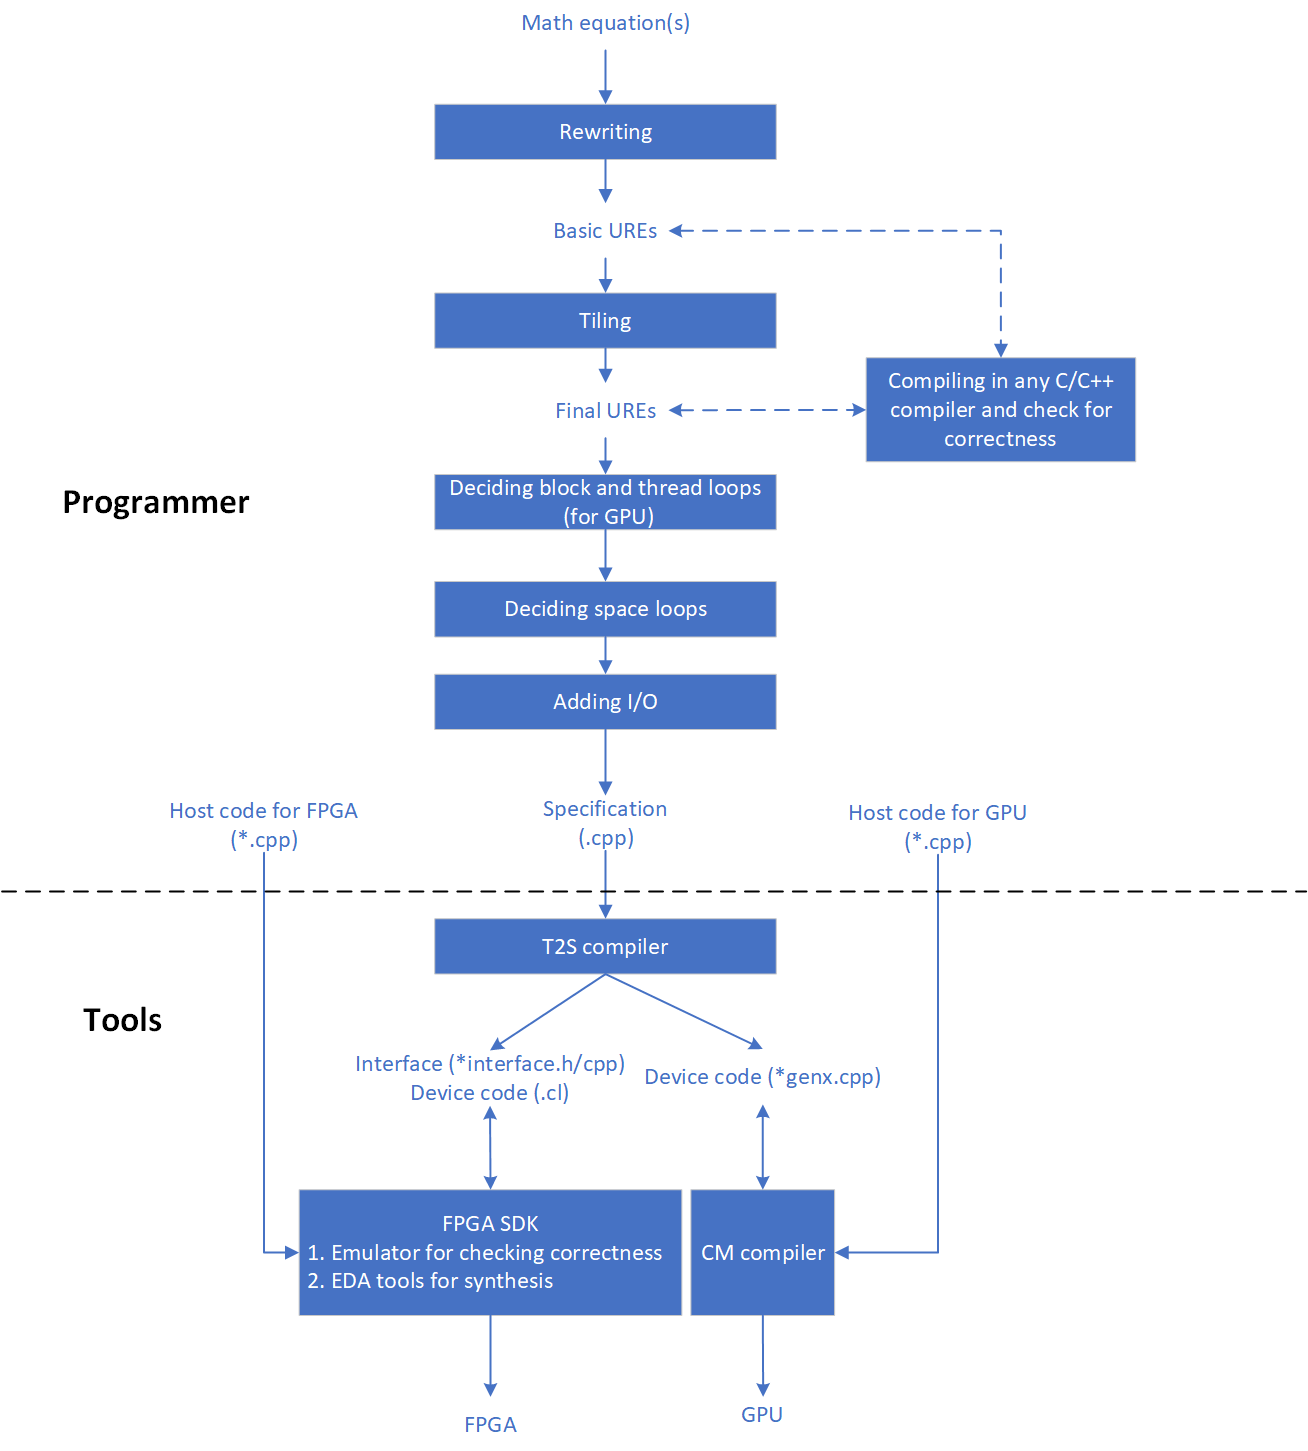
\includegraphics[width=\textwidth]{img/overall-flow.png}
    \caption{Overall flow}
    \label{fig:overall-flow}
\end{figure}

\chapter{Rewriting math equations into basic UREs}

Based on the work of Gusev and Evans~\cite{broadcastElim,broadcastElimQR},  we can translate math equations into UREs, following the simple steps below. Going through an example, we would find that this process is pretty much mechanical and intuitive, and only middle-school level of math knowledge is needed. So do not be scared by the math symbols. In fact, you want to work out the UREs through the simple math process, since the correctness can be proved and that would save you time in debugging.

We strongly recommend a beginner repeats the steps of an example, during which the beginner would quickly master the skills. These skills are applicable to other real world problems, not limited to the examples here.

Use auto-regressive filter~\cite{autoRegressiveModel} for example:
\begin{equation}
 X_t=c+\sum\limits^p_{i=1}\varphi_i X_{t-i}+\varepsilon_t
\end{equation}
where $c$ is a constant, $\varphi_1, ... \varphi_p$ are the parameters, $\varepsilon _t$ is white noise, and $X_t$ is the output at the current time $t$ and is dependent on the previous $p$ outputs $ X_{t-1}, ..., X_{t-p}$. 

This table shows the complete progress how UREs are derived for the problem, and the steps are explained in more detail below:

\begin{table*}[!ht]
\begin{tabular}{|l|ll|ll|}
\hline
    \multicolumn{1}{|c|}{\textbf{Step}} & \multicolumn{2}{|c|}{\textbf{Equations}} & \multicolumn{2}{|c|}{\textbf{Initial values}} \\\hline\hline
     \multirow{1}{*}{1: Iterative form}
        & $X_t=c+\sum\limits^p_{i=1}\varphi_i X_{t-i}+\varepsilon_t$    & $t=1, ..., n$   & $X_{t-i}=0$ &if $t-i \le 0$          \\\hline
     \multirow{2}{*}{2: Recursive form}
        & $X_t=X_t+\varphi_i X_{t-i}$                   & $t=1,...,n$ & $X_t=c+\varepsilon_t$ &  \\
        &                                         &   $i=1,..,p$      &  $X_{t-i}=0$ &if $t-i \le 0$ \\\hline        
     \multirow{2}{*}{3: DSA}
        & $X_t^i=X_t^{i-1}+\varphi_i X_{t-i}^p$         & $t=1,...,n$  & $X_t^{0}=c+\varepsilon_t$ & \\
        &                                         &  $i=1,..,p$& $X_{t-i}^p=0$ &if $t-i \le 0$\\\hline        
     \multirow{2}{*}{4: Full index form}
         & $X_t^i=X_t^{i-1}+\varphi_i^0 X_{t-i}^p$      & $t=1,...,n$ & $X_t^{0}=c+\varepsilon_t^0$  & \\
         & &$i=1,..,p$ & $X_{t-i}^p=0$ &if $t-i \le 0$\\\hline         
     \multirow{4}{*}{5: UREs}
         & $\Phi_t^i=\Phi_{t-1}^i$             && $\Phi_{0}^i=\varphi_i^0$  & \\
         & $\chi_t^i=\chi_{t-1}^{i-1}$         && $\chi_{t-1}^{i-1}=X_{t-i}^p$ &if $t-1=0$ or $i-1=0$ \\
         & $X_t^i=X_t^{i-1}+\Phi_t^i\chi_t^i$ &$t=1,...,n$ & $X_t^{0}=c+\varepsilon_t^0$ &\\
         & & $i=1,..,p$& $X_{t-i}^p=0$ &if $t-i \le 0$\\\hline         
\end{tabular}
\caption{Deriving UREs for auto-regressive filter}
\label{tab:deriving-ures-for-auto-regressive-filter}
\end{table*}


\section{Step 1: Iterative form}

First, write down the math equation(s) of the original problem. Usually, in an  equation, a domain  is iterated (like $i=1,...,p$ and $t=1,...,n$),  and some variable (like $X$) is computed. A variable might have some initial values (like $X_{t-i}=0$ for $t-i \le 0$) before the iteration starts.

\section{Step 2: Recursive form}

Translating the iterative form to a recursive form is straightforward: according to the iterative form, initialize a variable (e.g. $X_t=c+\varepsilon_t$), and update the variable every iteration with a new value based on its previous value (e.g. $X_t=X_t+...$).

\section{Step 3: DSA (Dynamic Single Assignment)}

When updating a variable every iteration, save it to a distinct memory location. Every reference to a variable thus exposes the iteration in which the variable is defined. For example, $X_t=X_t+...X_{t-i}$ is changed into  $X_t^i=X_t^{i-1}+...X_{t-i}^p$. After this renaming, it is clear that the 3 references to $X$ are referring to the $X$ values defined in the current iteration $\begin{psmallmatrix}i\\t\end{psmallmatrix}$ and previous iterations $\begin{psmallmatrix}i-1\\t\end{psmallmatrix}$ and $\begin{psmallmatrix}p\\t-i\end{psmallmatrix}$, respectively. 
Consequently, dataflow/dependences between these iterations are made explicit.  

For another example, the initialization $X_t=c+\varepsilon_t$ is changed into  $X_t^0=c+\varepsilon_t$ by adding one 0 for the missing index $i$. $X_t^0$ refers to the $X$ value defined in iteration $\begin{psmallmatrix}0\\t\end{psmallmatrix}$, which is outside the domain, because index $i$ starts from 1 with a step of 1. In general, if index $i$ starts from $s$ with a step $h$, the initial value should be $X_t^{s-h}$.

\section{Step 4: Full index form}

Now variables are referenced with full indices, but constants are not: $\varphi_i$ and $\varepsilon_t$ are inputs never modified when computing $X_t$ (The other constant $c$ is just a number and we do not care). Similar to the handling of initialization in step 3, we give these constants full indices by adding 0's for the missing index $i$:  change $\varphi_i$ and $\varepsilon_t$  into $\varphi_i^0$ and $\varepsilon_t^0$. They refer to the $\varphi$ and $\varepsilon$ values defined in iteration $\begin{psmallmatrix}0\\i\end{psmallmatrix}$ and $\begin{psmallmatrix}0\\t\end{psmallmatrix}$, respectively,  which are outside the domain. In general, if iteration index $i$ starts from $s$ with a step $h$, we should rename $\varphi_i$ and $\varepsilon_t$ into $\varphi_i^{s-h}$ and $\varepsilon_t^{s-h}$.

After being full indexed, variables and constants will be processed in the same way.

At this point, the equations we get are AREs (Affine Recurrence Equations), that is, the current iteration $\begin{psmallmatrix}i\\t\end{psmallmatrix}$ reads a value defined in a previous iteration with a distance $d$ that is in the form of  $d=A\begin{psmallmatrix}i\\t\end{psmallmatrix}+d_0$, where $A$ is a matrix and $d_0$ a constant vector. In other words, there is a read-after-write affine dependence between the two iterations. The dependence distance can be calculated as the current iteration  - the previous iteration  = the write's index - the read's index: Remember that every write/read is fully indexed with the iteration that defines its value; thus the write is indexed with the current iteration, the read is indexed with the previous iteration.  See Table~\ref{tab:deps-full-index-form-auto-regressive-filter} for all the dependences:

\begin{table*}[!ht]
\begin{tabular}{|c|c|c|l|}
\hline
    \multicolumn{1}{|c|}{\textbf{Dependence No.}} & \multicolumn{1}{|c|}{\textbf{Write}} & \multicolumn{1}{|c|}{\textbf{Read}} & \multicolumn{1}{|c|}{\textbf{Dependence distance}}\\\hline\hline
     \multirow{1}{*}{1} & $X_t^i$ & $X_t^{i-1}$ &  $\begin{pmatrix} i\\t\end{pmatrix} -  \begin{pmatrix} i-1 \\ t\end{pmatrix} =  \begin{pmatrix} 1 \\ 0\end{pmatrix}$ \\\hline
     \multirow{1}{*}{2} & $X_t^i$ & $\varphi_i^{0}$ &  $\begin{pmatrix} i\\t\end{pmatrix} -  \begin{pmatrix} 0 \\ i \end{pmatrix} =  \begin{pmatrix} i \\ t-i\end{pmatrix} =  \begin{pmatrix} 1 & 0 \\ -1 & 1\end{pmatrix}  \begin{pmatrix} i \\ t\end{pmatrix}$ \\\hline
     \multirow{1}{*}{3} & $X_t^i$ & $X_{t-i}^{p}$ &  $\begin{pmatrix} i\\t\end{pmatrix} -  \begin{pmatrix} p \\ t-i \end{pmatrix} =  \begin{pmatrix} i-p \\ i\end{pmatrix} =  \begin{pmatrix} 1 & 0 \\ 1 & 0\end{pmatrix}  \begin{pmatrix} i \\ t\end{pmatrix} + \begin{pmatrix} -p \\ 0 \end{pmatrix}$  \\\hline
\end{tabular}
\caption{Dependences of the full index form in  step 4 in Table~\ref{tab:deriving-ures-for-auto-regressive-filter}}.
\label{tab:deps-full-index-form-auto-regressive-filter}
\end{table*}

\section{Step 5: UREs}

We translate AREs into UREs by converting a broadcast into a pipeline. After that, every dependence has a constant distance uniformly in the entire domain.

There are two ways to convert a broadcast into a pipeline, either graphically or mathematically. 

\subsection{First way to translate AREs into UREs: drawing a dataflow graph}
\label{sec:are-to-ures-with-dfg}

We can draw the dataflow and intuitively figure out how to change a broadcast into a pipeline, as exemplified in Fig.~\ref{fig:broadcast-to-pipeline-arf}. According to the 2nd dependence in Table~\ref{tab:deps-full-index-form-auto-regressive-filter}, originally, a datum $\varphi_i^0$ is broadcast to iterations $X_t^i$ for all $i$, as shown in the left of the figure. 

Equivalently, the same datum can be loaded in an iteration at a boundary of the domain, and from that iteration, propagated in a pipeline fashion to all the other iterations, as shown in the right of the figure. As we can see, $\varphi_i^0$ is  loaded at a bounary iteration $(i, 1)$, and then is propagated to iteration $(i, 2)$, and from there to iteration $(i, 3)$, etc. 

\begin{figure}[!ht]
    \centering
    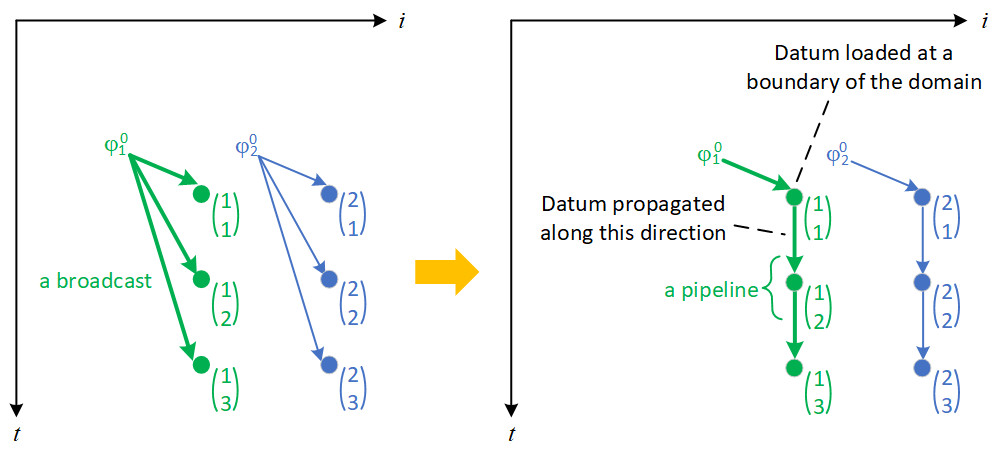
\includegraphics[width=\textwidth]{./img/broadcast-to-pipeline-arf.png}
    \caption{For the 2nd dependence of auto-regressive filter in Tabel~\ref{tab:deps-full-index-form-auto-regressive-filter}, the broadcasts due to this dependence are changed to pipelines. Here we assume $n=3$, and every point is an iteration annotated with its indices $\begin{psmallmatrix} i\\ t\end{psmallmatrix}$.}
    \label{fig:broadcast-to-pipeline-arf}
\end{figure}

\subsubsection{Expressing a pipeline} 
\label{sec:express-pipeline}

Now we can modify the full index form

\begin{equation}
X_t^i=...\varphi_i^0...
\end{equation}

into

\begin{equation}
X_t^i=...\Phi_t^i...
\end{equation}

where $\Phi$ values are propagated along the $t$ dimension:

\begin{equation}
\Phi_t^i=\Phi_{t-1}^i
\end{equation}

until out of the domain:
\begin{equation}
\Phi_0^i=\varphi_i^0
\end{equation}

As you can say, the keys to change a broadcast into a pipeline are: (1) the direction of the pipeline, along which data would be propagated from one iteration to the next, and (2) the initial value defined by one iteration that is  out of the domain.  

In the same way, we can convert a broadcast due to the third dependence into a pipeline (Could you do it?). After that, we get the UREs shown in step 5 of  Table~\ref{tab:deriving-ures-for-auto-regressive-filter}.

\subsection{Second way to translate AREs into UREs: Calculating a propagation direction}
\label{sec:are-to-ures-with-math}

We can generalize the example in Fig.~\ref{fig:broadcast-to-pipeline-arf}, and directly find out a propagation direction vector in simple math: 

\begin{quotation}
\noindent If a read-after-write dependence is affine, i.e. the distance $d$ is in the form of $Az+d_0$, where $A$ is a matrix, $z$ is the current iteration, and $d_0$ is a constant vector, then the dependence incurs broadcasts of values, and such a broadcast can be changed into a pipeline by propagating a value along a direction $r$ that is a solution of $(I-A)r=\mathbf{0}$, where $I$ is the identity matrix.
\end{quotation}

\begin{figure}[!ht]
    \centering
    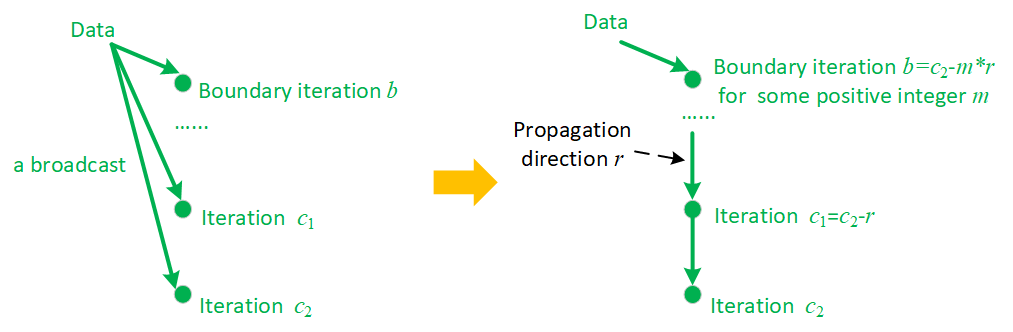
\includegraphics[width=\textwidth]{./img/broadcast-to-pipeline.png}
    \caption{Changing a broadcast into a pipeline}
    \label{fig:broadcast-to-pipeline}
\end{figure}

The left part of Fig.~\ref{fig:broadcast-to-pipeline} shows that due to an affine dependence, some data are broadcast to multiple consumers, including an iteration $b$ at the boundary of the domain, and two other iterations $c_1$ and $c_2$, etc. Remember that data are fully indexed, i.e. they can be considered having been defined in an iteration $y$, even though that iteration is actually out of the domain. 

Let the dependence distance be $d=Az+d_0$.  Because both iteration $c1$ and $c_2$ get data from the same iteration $y$, using the  dependence distance, we have
\begin{equation}
y = c_2 - (Ac_2+d_0) = c_1 - (Ac_1+d_0)
\end{equation}

So
\begin{equation}
(I-A)c_2 = (I_A)c_1    
\end{equation}

Let $r=c_2-c1$, we have
\begin{equation}
(I-A)r = 0.
\end{equation}

Therefore, we can imagine that a datum that is defined outside the domain is first sent to a boundary iteration $b$, and then following a propagation direction $r$ to the next iteration $b+r$, and so on, and eventually the data reach iteration $c_1$, and then $c_2$, etc. This constructs a pipeline as shown in the right part of Fig.~\ref{fig:broadcast-to-pipeline}.

For example, the second dependence for the auto-regressive filter is $\begin{psmallmatrix} 1 & 0 \\ -1 & 1\end{psmallmatrix}  \begin{psmallmatrix} i \\ t\end{psmallmatrix}$ (Table~\ref{tab:deps-full-index-form-auto-regressive-filter}), and thus $A=\begin{psmallmatrix} 1 & 0 \\ -1 & 1\end{psmallmatrix}$. Solve the equation $(I-A)r=\begin{psmallmatrix} 0 & 0 \\ 1 & 0\end{psmallmatrix}=\mathbf{0}$. We get a solution $r=\begin{psmallmatrix} 0 &\\ *\end{psmallmatrix}$, where the second element (the $t$ dimension)  can be arbitrary. Take a non-zero solution $r=\begin{psmallmatrix} 0 &\\ 1\end{psmallmatrix}$, and we see exactly from the right part of Fig.~\ref{fig:broadcast-to-pipeline-arf} that a  pipeline can be constructed along the $t$ dimension for a datum. 

With this propagation direction, we convert a broadcast due to the second dependence into a pipeline in the same way as shown in Section~\ref{sec:express-pipeline}. Following the same approach, for the third dependence, we can find a propagation direction $r=\begin{psmallmatrix} 1 &\\ 1\end{psmallmatrix}$, and convert the broadcasts due to this dependence into pipelines as well (Could you do it?). After that, we get the UREs shown in step 5 of  Table~\ref{tab:deriving-ures-for-auto-regressive-filter}.

\subsection{Testing correctness of UREs}
\label{sec:test-correctness-ures}

We can test the correctness of UREs either in standard C or in T2S.

We can express the UREs in Table~\ref{tab:deriving-ures-for-auto-regressive-filter} in standard C, adding necessary helping code for testing, and see if the UREs can produce correct results:

\begin{listing}[htbp]
\caption{A specification for the algorithm in Fig.~\ref{fig:GEMM-explained}}
\label{lst:matrix-multiply-spec}
\vspace{-1ex}
\begin{minted}[fontsize=\footnotesize,]{cpp}
for (i = 1; i <= n; i++) {
  for (j = 1; j <= n; j++) {
    Prev_C(j, i) = (i==1) ? c(0, j) : C(j, i-1);
    Prev_Y(j, i) = (i==1 || j==1) ? y(n, i-j) : Y(j-1, i-1);
    C(j, i)      = Prev_C(j, i);
    Y(j, i)      = Prev_Y(j, i);
    y(j, i)      = y(j-1, i) + C(j, i)*Y(j, i);
  }
}

#define ATYPE Int(8, 10, 1)
#define BTYPE Int(8, 3, 10)
#define CTYPE Float(32, 3, 1)
// Inputs: 2-dimensional tensors (i.e. matrices)
ImageParam a(ATYPE, 2), b(BTYPE, 2);
// Loop variables
Var kkk, jjj, iii, jj, ii, kk, k, j, i;

/*************** Temporal Definition ***************/
// UREs
Func A(ATYPE, {P}, Place::Device), B(BTYPE, {P}, Place::Device),
     C(CTYPE, {P}, Place::Device), Result(Place::Device);
A(P)=select(jjj==0, a(total_k,total_i), A(P_jjj_minus_1));
B(P)=select(iii==0, b(total_j,total_k), B(P_iii_minus_1));
C(P)=select(kkk==0 && kk==0 && k==0, Zero(CTYPE),
            select(kkk==0 && kk==0, C(P_k_minus_1), 
                   select(kkk==0,   C(P_kk_minus_1),
                                    C(P_kkk_minus_1)))
     ) + A(P) * B(P);
Result(P_result)=select(kkk==KKK-1 && kk==KK-1 && k==K-1, C(P));
// Put all the UREs into the same loop nest. 
// From now on, A represents all the UREs. 
A.merge_ures(B, C, Result);
// Explicitly set the loop bounds
A.set_bounds(kkk, 0, KKK, jjj, 0, JJJ, iii, 0, III,
                          jj,  0, JJ,  ii,  0, II,
             k,   0, K,   j,   0, J,   I,   0, I);

/***************** Spatial Mapping *****************/
// Create a systolic array
A.space_time_transform(jjj, iii);
// I/O Network
Stensor DA(DRAM), HA(HBM), SA(SRAM),
        DB(DRAM), HB(HBM), SB(SRAM),
        RC(REG),  DC(DRAM), c;
a>>DA.out(kkk)>>HA.scope(j).out(iii,ii,kkk)>>SA.scope(k).out(iii,kkk);
b>>DB.out(kkk)>>HB.scope(j).out(jjj,jj,kkk)>>SB.scope(k).out(jjj,kkk);
Result>>RC.scope(iii).out(jjj)>>DC>>c(total_j,total_i);

Buffer<CTYPE> c_buf(JJJ*JJ*J, III*II*I);
c.realize(c_buf, IntelFPGA);
\end{minted}
\vspace{-5ex}
\end{listing}

\chapter{Writing tiled UREs}
TBD.
\chapter{Multi-threading}
TBD.
\chapter{Building a systolic array}
TBD.
\chapter{How to compile and run}
\label{cha:compile-and-run}

Suppose a specification file, named \texttt{a.cpp}, is ready, and it contains such statements:
    \begin{markdown}
        Func SomeKernel(Place::Device);
        definition of SomeKernel
        SomeKernel.compile_to_host("interface", parameters of SomeKernel, IntelFPGA);
    \end{markdown}

And suppose a host file \texttt{host.cpp} is ready to call \texttt{SomeKernel}.

\begin{enumerate}
\item {\bf Set up environment}.
    
    Under the T2SP root directory:
    \begin{markdown}
    source setenv.sh (local | devcloud) fpga
    \end{markdown}
    
    \item {\bf Compile the specification}.
    \begin{markdown}
    # If you intend to emulate your design on a CPU:
    g++ a.cpp $COMMON_OPTIONS_COMPILING_SPEC $EMULATOR_LIBHALIDE_TO_LINK
    
    # Or if you intend to execute it on real FPGA hardware:
    g++ a.cpp $COMMON_OPTIONS_COMPILING_SPEC $HW_LIBHALIDE_TO_LINK
    \end{markdown}

    \item {\bf Run the specification to generate the kernel}.
    \begin{markdown}
    # For emulation:
    env BITSTREAM=a.aocx AOC_OPTION="$COMMON_AOC_OPTION_FOR_EMULATION" ./a.out    
    
    # Or for execution:
    env BITSTREAM=a.aocx AOC_OPTION="$COMMON_AOC_OPTION_FOR_EXECUTION" ./a.out    
    \end{markdown}
    For the kernel, this command generates an OpenCL file (named \texttt{a.cl} after name of the environment variable \texttt{BITSTREAM}), invokes Intel FPGA SDK for OpenCL to synthesize the OpenCL file into a device bitstream (\texttt{a.aocx}), and generates \texttt{interface.h/cpp} for the host to invoke the kernel, as if the kernel is a common CPU function.

    You may modify the generated OpenCL file manually. A common debugging practice is to add \texttt{printf} statements inside the generated OpenCL file, e.g. inserting \texttt{printf("Variable v=\%f", v)} to dump the value of variable \texttt{a}. Note \texttt{printf} works only with emulation.
    
    After any modification, you may re-generate the bitstream in the following commands:
    \begin{markdown}
    # For emulation:
    aoc $COMMON_AOC_OPTION_FOR_EMULATION a.cl -o a.aocx    
    
    # Or for execution:
    rm -rf a.aoc* a/
    aoc $COMMON_AOC_OPTION_FOR_EXECUTION a.cl -o a.aocx    
    \end{markdown}

    \item{\bf Compile the host file}
    \begin{markdown}
    # For emulation:
    g++ host.cpp interface.cpp $COMMON_OPTIONS_COMPILING_HOST_FOR_EMULATION -o host.out
    
    # Or for execution:
    g++ host.cpp interface.cpp $COMMON_OPTIONS_COMPILING_HOST_FOR_EXECUTION -o host.out
    \end{markdown}
    When compiling the host file, the kernel will be linked to the host code through the interface.

    \item {\bf Run the host file}
    \begin{markdown}
    # For emulation:
    env BITSTREAM=a.aocx CL_CONTEXT_EMULATOR_DEVICE_INTELFPGA=1 \
        INTEL_FPGA_OCL_PLATFORM_NAME="$EMULATOR_PLATFORM" ./host.out

    # For execution:
    # DevCloud A10PAC FPGA only: convert the signed bitstream to be unsigned first
    #   Type `y` when prompted
        source $AOCL_BOARD_PACKAGE_ROOT/linux64/libexec/sign_aocx.sh \ 
               -H openssl_manager -i a.aocx -r NULL -k NULL -o a_unsigned.aocx
        mv a_unsigned.aocx a.aocx
    # Offload and run    
    aocl program acl0 a.aocx
    env BITSTREAM=a.aocx INTEL_FPGA_OCL_PLATFORM_NAME="$HW_PLATFORM" ./host.out
    \end{markdown}
    
    \item {\bf Debug a kernel (in an emulator only)}
    
    Just like debugging any executable in \texttt{gdb}, you would like to add \texttt{gdb} right before \texttt{./host.out}:
    \begin{markdown}
    env BITSTREAM=a.aocx CL_CONTEXT_EMULATOR_DEVICE_INTELFPGA=1 \
        INTEL_FPGA_OCL_PLATFORM_NAME="$EMULATOR_PLATFORM" gdb ./host.out

    # Now inside the gdb, set a breakpoint at the kernel
    (gdb) b SomeKernel
    
    # Run. Gdb will stop at the kernel's entrance.
    (gdb) r
    \end{markdown}
    
    Note: whether \texttt{gdb} could successfully stop at the specified kernel seems to depend on the version of \texttt{aoc} (i.e. Intel FPGA SDK for OpenCL). We verified that the debugger stops at a kernel with aoc 19.2.0 on an S10 FPGA, but somehow does not stop with aoc 19.4.0 on an A10 FPGA.
\end{enumerate}

Note: if you want to re-run the above commands, remove the previously generated bitstream and intermediate files:
    \begin{markdown}
        rm -rf a.* a/ *interface.* *.out exec_time.txt
    \end{markdown}
\bibliographystyle{plain}
\bibliography{references}



\end{document}